\documentclass[preprint]{article}

\usepackage{neurips_2023}
\usepackage[authoryear]{natbib}

\usepackage{bookmark}
\usepackage[utf8]{inputenc}
\usepackage[T1]{fontenc}
\usepackage{hyperref}
\usepackage{url}
\usepackage{booktabs}
\usepackage{amsfonts}
\usepackage{nicefrac}
\usepackage{microtype}
\usepackage{xcolor}
\usepackage{listings}
\usepackage{cite}
\usepackage{graphicx}
\usepackage{amsmath}
\usepackage{algpseudocode}
\usepackage{algorithm}
\usepackage{caption}
\usepackage{pdflscape}
\usepackage{tabularx}
\usepackage{multirow}
\usepackage{float}
\usepackage{adjustbox}

% The default skips put a caption flush against its table and a float flush against the
% surrounding text, which reads as a wall.
\setlength{\abovecaptionskip}{10pt}
\setlength{\belowcaptionskip}{8pt}
\setlength{\textfloatsep}{22pt plus 4pt minus 4pt}
\setlength{\intextsep}{22pt plus 4pt minus 4pt}
\setlength{\floatsep}{20pt plus 4pt minus 4pt}

\hypersetup{
pdftitle={How to Reduce Whisper Hallucination},
pdfauthor={Husein Zolkepli},
pdfsubject={Audio and Speech Processing},
pdfkeywords={speech recognition, hallucination, whisper, fine-tuning},
colorlinks=true,
linkcolor=blue,
citecolor=blue,
urlcolor=blue
}
\title{How to Reduce Whisper Hallucination}
\author{
  Husein Zolkepli \\
  Scicom (MSC) Berhad, Malaysia \\
  \texttt{husein.zolkepli@scicom.com.my}
}

\begin{document}

\maketitle

\begin{abstract}
Whisper is still the best open multilingual speech recogniser available. It is also the one
that writes sentences nobody said. On 42 clips of pure room tone, \texttt{whisper-large-v3}
emits words on 61.9\% of them and emits something on 100\% of them. The usual response is to
distil a student from Whisper pseudo-labels and filter the hallucinations out of the corpus
first. That removes the evidence, not the behaviour: the student is fitted to the subset where
the teacher was right, so it inherits a failure mode that never appears in its own training
data. The second response, adding non-speech audio so the model learns to stay quiet, is
already used in production systems and it works, but it teaches suppression without teaching
discrimination. The checkpoint that is best on every non-speech arm here is also the one that
recovers the fewest genuinely spoken phrases and deletes 58\% of repeated speech. We argue the
teacher has to be fixed, with both halves of the signal, and we do the work that requires. We build a
benchmark that scores both halves of the problem at once, 11,852 clips over eight arms plus
6,267 synthetic positives, 8,296 clips of real audio that made a production model fail, and
FLEURS in 58 languages. We collect a lexicon of 40,891 hallucination phrases in 100 languages,
select a text-to-speech system by measurement rather than reputation, and synthesise those
phrases as positives so the model sees the same text both as something to suppress and as
something to transcribe. We then sweep fine-tuning over rank, learning rate, and the presence
of the synthetic positives. The benchmark, the lexicon and the synthetic corpus are released at
\href{https://huggingface.co/datasets/Scicom-intl/Whisper-Hallucination}{Scicom-intl/Whisper-Hallucination}.
\end{abstract}

\section{Introduction}

Whisper \citep{radford2022whisper} is the model to beat in open multilingual speech
recognition. One checkpoint covers 99 languages, runs anywhere, and needs no per-language
tuning. We measured it on 20 FLEURS \citep{conneau2022fleurs} test clips in each of 58
languages: \texttt{whisper-large-v3} reaches a character error rate of 0.075 on the typical
language, and 35 of the 58 languages land under 0.15. Nothing else open is close on that
combination of coverage and accuracy.

It also invents text. Not rarely, not only on hard audio, and not harmlessly.
\citet{koenecke2024careless} ran more than 13,000 clips from AphasiaBank through Whisper and
found that roughly 1\% of transcriptions contained entire hallucinated phrases or sentences
present nowhere in the audio, and that 38\% of those hallucinations carried explicit harms:
perpetuating violence, inventing associations, or implying false authority. Hallucination rates
were higher for speakers with longer non-vocal pauses, which is a symptom of aphasia, so the
failure is not distributed evenly across speakers.
\citet{baranski2025nonspeech} come at the same problem from the audio side and show that a
curated list of common hallucinations works as a post-processing filter. A recogniser that
writes a plausible sentence over silence is worse than one that returns an error, because
nothing downstream can tell the difference.

\begin{table}[tb]
\centering
\caption{Hallucination on audio that contains no speech. The correct output is the empty
string, so any output at all is wrong. The first block counts outputs containing words, the
second counts any output including a bare full stop.}
\label{tab:nonspeech}
\small
\begin{tabular}{lrrrrrr}
\toprule
\textbf{arm} & \textbf{n} & \textbf{large-v2} & \textbf{large-v3} & \textbf{turbo} & \textbf{malaysian-v2} & \textbf{M-turbo-v3} \\
\midrule
\texttt{silence} & 42 & 85.7\% & 61.9\% & 59.5\% & 35.7\% & \textbf{16.7\%} \\
\texttt{music} & 600 & 98.7\% & 97.0\% & 96.7\% & 69.7\% & \textbf{31.0\%} \\
\texttt{nonspeech} & 1{,}168 & 98.8\% & 89.9\% & 80.7\% & 76.0\% & \textbf{9.3\%} \\
\midrule
\texttt{silence} any output & 42 & 100\% & 100\% & 100\% & 64.3\% & \textbf{16.7\%} \\
\texttt{music} any output & 600 & 100\% & 100\% & 100\% & 73.0\% & \textbf{31.7\%} \\
\texttt{nonspeech} any output & 1{,}168 & 100\% & 100\% & 100\% & 77.8\% & \textbf{9.4\%} \\
\bottomrule
\end{tabular}
\end{table}

Every OpenAI checkpoint writes something on every single clip that has no speech in it. Read
the first block and the second block together, because published hallucination rates for the
same model on the same audio differ by more than ten times depending on which one an author
chose to report.

The second failure is repetition. On 1,440 clips built from a known unit repeated a known
number of times, the 95th percentile of emitted repeats divided by true repeats is 1.00 for
\texttt{large-v3} and 18.3 for \texttt{turbo}. The two Malay fine-tunes reach 55.0 and 73.3.
A single clip can produce hundreds of copies of one token.

Both failures come from the same place. The Whisper decoder is a language model conditioned on
an audio encoder. When the acoustic evidence is weak or absent, the prior takes over and the
decoder writes fluent text, because writing fluent text is what it was trained to do. Silence
is not a token it can emit. It has to decide to stop, and stopping is exactly what it is worst
at.

The field's response has been to work around the model. Put a voice activity detector in front
of it, threshold on \texttt{no\_speech\_prob}, block a list of known phrases after the fact.
All of these help, and none of them change the weights. Move to a serving stack that does not
implement Whisper's own decoding loop, which is what happens in production, and most of the
knobs disappear. vLLM exposes no \texttt{no\_speech\_threshold}, no
\texttt{compression\_ratio\_threshold}, no \texttt{logprob\_threshold}, and no
\texttt{condition\_on\_previous\_text}. What is left is the model.

\section{Distilling from Whisper}

The standard way to get a cheaper or a more multilingual Whisper is to run Whisper over
unlabelled audio, keep the transcripts, and train a student on them. The pipelines are public
and so are the filters, which is what makes this arguable rather than speculative.

Distil-Whisper \citep{gandhi2023distilwhisper} pseudo-labels with Whisper and then, in its own
words, uses ``a simple word error rate heuristic'' to select only the highest quality
pseudo-labels for training. Kotoba-Whisper \citep{kotobawhisper2024} applies the same recipe to
Japanese with \texttt{large-v3} as the teacher. NVIDIA's Granary
\citep{koluguri2025granary} builds a 25 language corpus with a pseudo-labeling pipeline whose
stages are listed as ``segmentation, two-pass inference, hallucination filtering, and
punctuation restoration'', and Canary-1B-v2 and Parakeet-TDT-0.6B-v3
\citep{sekoyan2025canaryv2} are trained on it.

Read those two descriptions next to each other. A hallucination filter is a device for removing
the teacher's hallucinations from the student's training set. It works. The corpus comes out
cleaner, and the resulting models are strong. But the examples it deletes are precisely the
ones that demonstrate the failure, so the student is fitted to the subset of the teacher's
behaviour that was already correct. It never sees a clip where the teacher wrote
\texttt{thank you for watching} over a music bed. It has no way to learn that this is wrong. It
learns the teacher's mapping on clean speech and inherits the teacher's prior everywhere else.

There is a second, quieter effect. Pseudo-label pipelines are built from speech corpora, and
speech corpora are segmented to speech. A clip with no voice in it yields a pseudo-label that
looks like garbage, so the filter drops it, or it was never in the corpus in the first place.
The student therefore has close to zero training examples whose correct output is the empty
string. Asking it to say nothing at inference time is asking for behaviour with no support in
its training distribution.

We measured how strongly segmentation hides this. GigaSpeech \citep{chen2021gigaspeech} is
podcasts and YouTube, which is the right material, and mining it for hallucinations yields
0.41\% of clips. AudioSet \citep{gemmeke2017audioset}, the same kind of source but unsegmented,
yields 54.70\%. The failures live in what segmentation throws away.

\subsection{Negative-only training}

The obvious remedy is to put non-speech audio back in. Two groups already do.

Canary-1B-v2 \citep{sekoyan2025canaryv2} states it plainly: the training mix has ``non-speech
audio added to reduce hallucinations for ASR and AST''. Mesolitica's Malaysian Whisper
fine-tunes \citep{mesolitica2025malaysianwhisper} do the same thing and, unusually, publish the
whole pipeline. Their stage-two training set includes an AudioSet block with a dedicated noise
subset, and the preparation code is open.

It works, and our benchmark shows exactly how well. In Table~\ref{tab:nonspeech},
\texttt{Malaysian-turbo-v3} is the best checkpoint measured on every non-speech arm, by a wide
margin: 16.7\% on silence against 61.9\% for base \texttt{large-v3}, and 9.3\% on non-speech
against 89.9\%. Adding negatives is not a marginal trick. It is the single most effective thing
anyone in this table did.

Then look at what it cost. The same checkpoint recovers 41.1\% of phrases that are genuinely
spoken, against 69.8\% for the base model it was tuned from (Table~\ref{tab:lexsynth}), deletes
58.0\% of clips containing repeated speech, and returns character error rate 1.26 on the typical
FLEURS language. It did not learn to detect silence. It learned a prior against emitting text,
and that prior fires on real speech too.

This is the gap we set out to close. Negative-only supervision teaches suppression without
teaching discrimination. The missing ingredient is audio that genuinely contains the phrases the
negatives are teaching the model to suppress: a recording where somebody really does say
\texttt{thank you for watching}, labelled with that transcript. No public pipeline has one,
because nobody collected the phrases first. So the fix has to be applied to the teacher, and it
has to supply both halves.

\section{Requirements}

Three things, in order.

\textbf{A benchmark that scores both halves.} A model that emits nothing is perfect on every
non-speech arm and useless. Any metric that looks only at hallucination will select it. The
benchmark has to measure suppression and accuracy on the same axis, on the same run.

\textbf{Knowledge of what the model actually says.} Hallucinations are not random. They are a
small set of phrases the model falls back on, and they differ by language. That set is
enumerable, and once enumerated it can be turned into training data.

\textbf{Training data where both answers appear.} The model needs clips whose correct output is
the empty string, and it needs clips where the very same phrases are genuinely spoken and must
be transcribed. Without the second half, suppression is learned as a blanket prior against
emitting text, which is the failure mode of every aggressive fine-tune we measured.

\section{Dataset}

\subsection{Non-speech audio}

\begin{table}[tb]
\centering
\caption{The eight benchmark arms. Every arm is a \texttt{test} split. The training corpus is a
separate build that is disjoint by construction, verified before any training run.}
\label{tab:arms}
\small
\begin{tabular}{llrl}
\toprule
\textbf{arm} & \textbf{source} & \textbf{clips} & \textbf{correct output} \\
\midrule
\texttt{silence} & 6 noise floors $\times$ 7 durations & 42 & nothing \\
\texttt{music} & Free Music Archive \citep{defferrard2017fma} & 600 & nothing \\
\texttt{nonspeech} & FSD50K \citep{fonseca2020fsd50k}, label-verified voice-free & 1{,}168 & nothing \\
\texttt{reduplication} & a unit repeated an exact number of times & 1{,}440 & that many repeats \\
\texttt{speech\_in\_noise} & genuine speech mixed at 5 SNRs & 1{,}200 & the transcript \\
\texttt{genuine} & real Malaysian speech & 4{,}694 & the transcript \\
\texttt{genuine\_isolated} & one phrase spoken alone & 88 & the phrase \\
\texttt{librispeech\_test\_clean} & LibriSpeech \citep{panayotov2015librispeech} & 2{,}620 & the transcript \\
\bottomrule
\end{tabular}
\end{table}

The \texttt{reduplication} arm deserves a note, because it is the only arm where both extremes
are wrong. A clip contains a unit repeated exactly $n$ times. Emitting more is runaway. Emitting
nothing is deletion. A metric that only penalises runaway will reward a model that deletes
repeated speech, and one of our own fine-tunes does exactly that.

\subsection{Spoken positives}

The negative arms ask what a model invents over silence. The positive arm asks what it does
when the same phrase is real. This is the half that stops the benchmark from selecting a mute
model, and it is built by synthesising the lexicon described in Section~\ref{sec:lexicon}.
It contains 29,112 clips in 83 languages, split into 22,845 train and 6,267 test.

Each test clip is scored three ways, because production audio arrives as a chunk with a noise
floor around it, not as a bare 0.9 second clip. The conditions are the clip as published, the
clip with two seconds of digital zeros on each side, and the clip with two seconds of real room
tone on each side drawn from the \texttt{silence} arm. The zeros condition is a control and
should do nothing, because Whisper pads every input to a 30 second window anyway.

\subsection{Wild audio}

Everything above is a built stimulus. The wild pool is real recordings that made a model fail:
3,607 Earnings-22 \citep{delrio2022earnings22} clips carrying human span annotations, 4,689
clips mined from streamed corpora with no annotator, and 187 aphasia clips kept local because
the source is membership-gated. It ships as 3,628 train and 4,668 test, split by source
recording rather than by clip, because a dozen segments can come from one call and a clip-level
split would leak near neighbours.

Mining needs no annotator. Two signatures are self-evident: a token run of six or more, and
words emitted where Silero voice activity detection finds no speech. We never call a clip a
hallucination because a transcript disagrees with a reference, since that finds ordinary
recognition errors.

\begin{table}[tb]
\centering
\caption{Hallucination yield by corpus, per 8,000 clips heard. Recording quality predicts yield
across five thousandfold.}
\label{tab:yield}
\small
\begin{tabular}{llrr}
\toprule
\textbf{corpus} & \textbf{character} & \textbf{kept} & \textbf{rate} \\
\midrule
AudioSet \citep{gemmeke2017audioset} & YouTube, heavy background noise & \textbf{4{,}376} & \textbf{54.70\%} \\
AMI \citep{carletta2005ami} & spontaneous meetings, far-field & 235 & 2.94\% \\
GigaSpeech \citep{chen2021gigaspeech} & podcasts and YouTube, speech-aligned & 33 & 0.41\% \\
Earnings-22 \citep{delrio2022earnings22} & conference calls & 31 & 0.39\% \\
People's Speech \texttt{dirty} \citep{galvez2021peoplesspeech} & noisy transcripts, clean audio & 9 & 0.11\% \\
VoxPopuli \citep{wang2021voxpopuli} & parliament & 4 & 0.05\% \\
People's Speech \texttt{clean} & curated read speech & 1 & 0.01\% \\
\bottomrule
\end{tabular}
\end{table}

Two lessons. Curated corpora barely fail, so a hallucination study built on them will conclude
the problem is small. And a corpus can be the right material and still hide the failure:
GigaSpeech is podcasts and YouTube and yields 0.41\%, because its segments are cut to speech.

\subsection{Multilingual accuracy}

\texttt{librispeech\_test\_clean} is English. A multilingual fine-tune can hold its English word
error rate and destroy everything else, and nothing in an English benchmark will show it. We
add a FLEURS arm: 20 test clips in each of 58 languages, averaged per language rather than per
clip so a large language cannot mask a collapsed one, and in character error rate because
Chinese, Japanese, Thai, Lao, Burmese and Khmer do not put spaces between words.

This arm paid for itself immediately, as Section~\ref{sec:bench} shows.

\section{Benchmark results}
\label{sec:bench}

Five checkpoints, greedy decoding, no forced language, no temperature fallback. Every
checkpoint is run on all of it, roughly 40,000 clips each.

Three are the OpenAI base models. The other two are Mesolitica's Malaysian fine-tunes, and they
are in the set for a reason: they are the closest public thing to the fix this paper proposes.
Their pipeline is open, their training mix already contains non-speech audio, and they are the
only checkpoints here that were deliberately tuned against hallucination. Treat them as the
strong baseline, not as a foil.

\begin{figure}[tb]
  \centering
  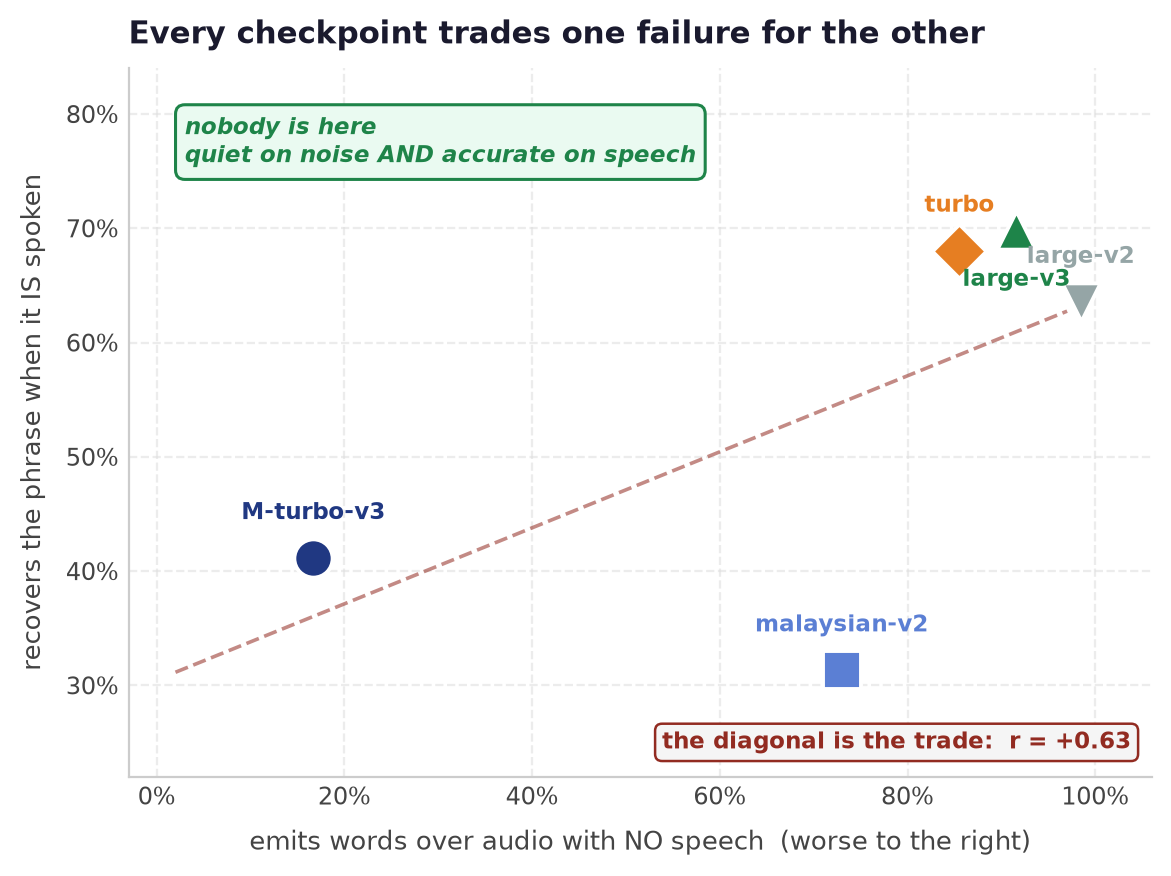
\includegraphics[width=0.86\linewidth]{img/fig_tradeoff.png}
  \caption{Every checkpoint trades one failure for the other. Horizontal axis is how often the model emits words over audio with no speech in it, pooled over the three non-speech arms and weighted by clip count. Vertical axis is how often it recovers a phrase that is genuinely spoken. The top left corner is the model everyone wants and nothing is there.}
  \label{fig:tradeoff}
\end{figure}

\textbf{No checkpoint is both quiet on noise and accurate on speech.} The five sit on a line,
$r = +0.63$ between the pooled non-speech word-emission rate and phrase recovery. Quiet models delete real speech and accurate models write over silence. This is
the central measurement of the paper and it is what makes a one-sided metric dangerous.

\begin{figure}[tb]
  \centering
  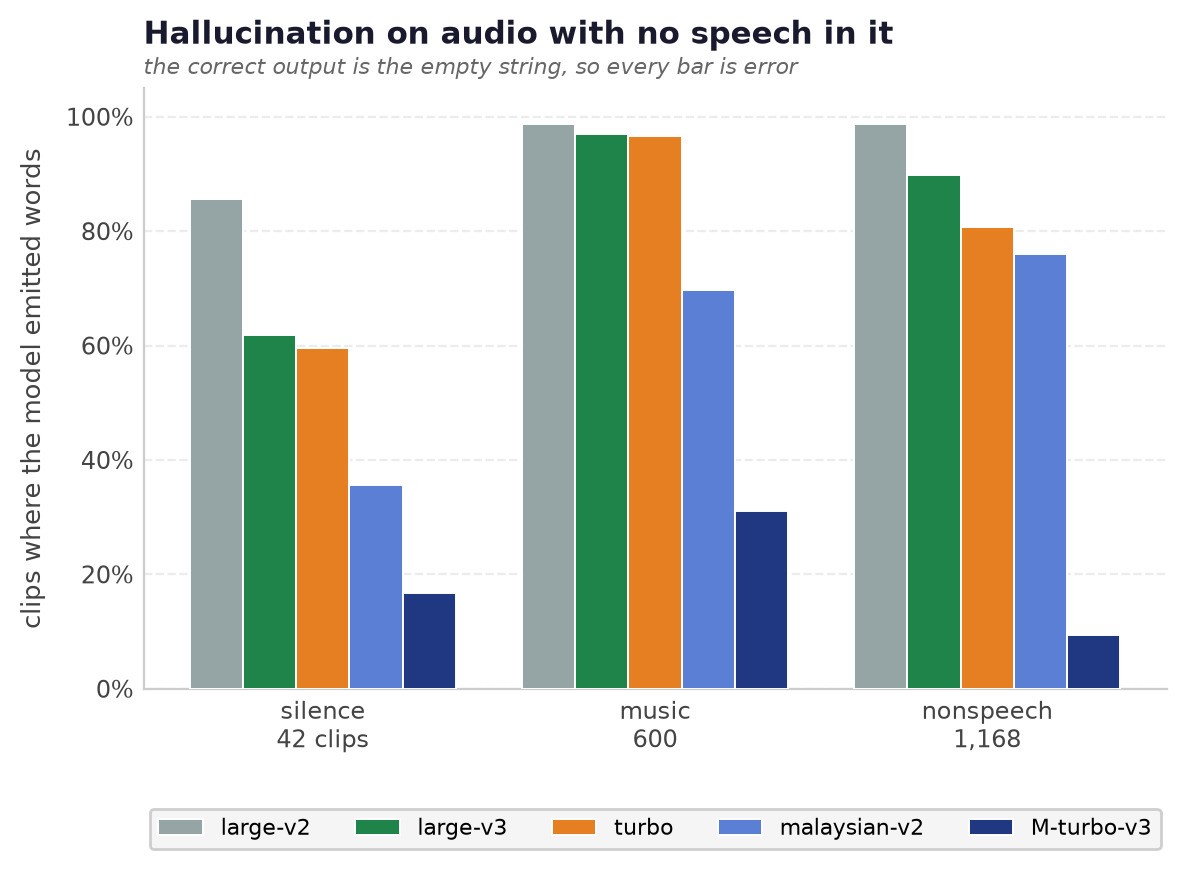
\includegraphics[width=0.86\linewidth]{img/fig_nonspeech.png}
  \caption{Hallucination on the three non-speech arms. Every bar is error, because the correct output is the empty string.}
  \label{fig:benchmark}
\end{figure}

\begin{figure}[tb]
  \centering
  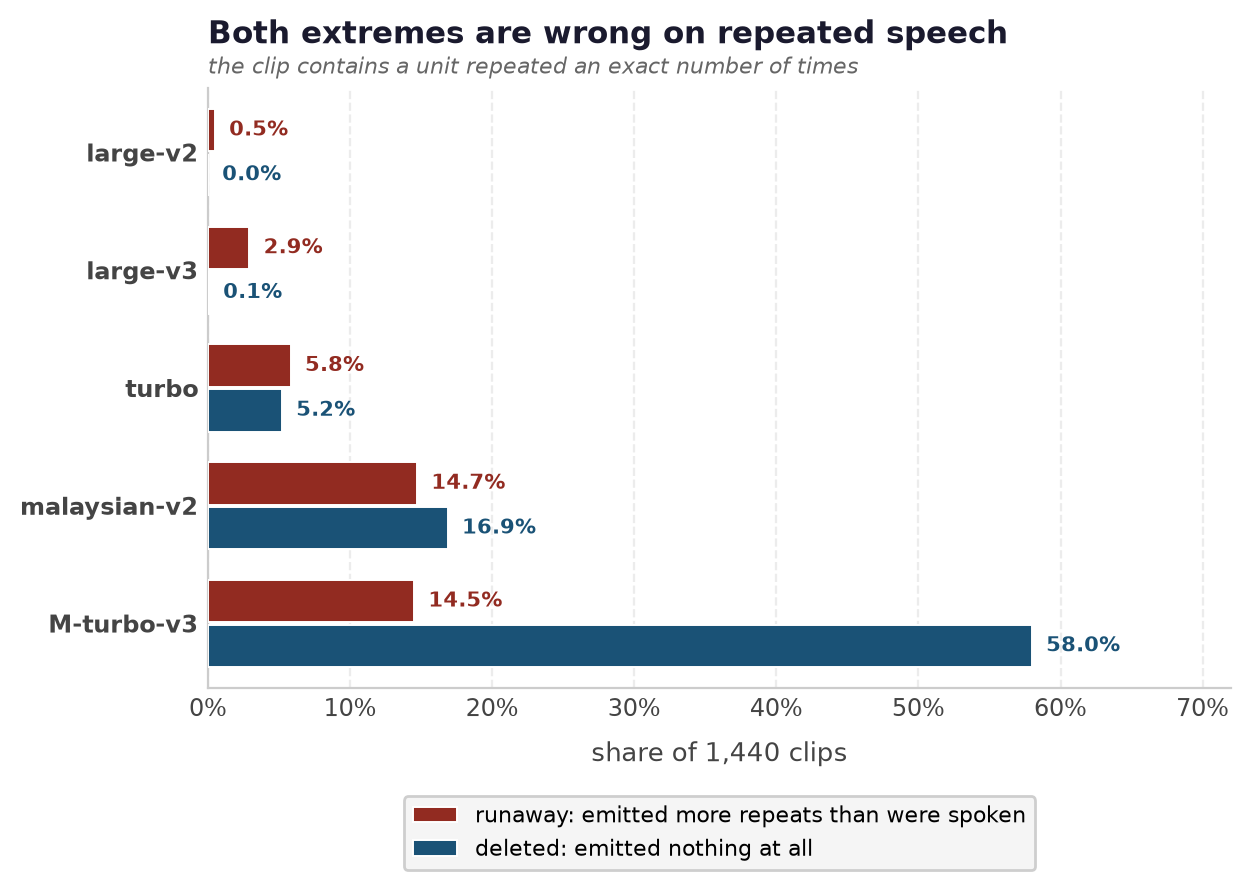
\includegraphics[width=0.86\linewidth]{img/fig_repetition.png}
  \caption{Both extremes are wrong on repeated speech. A model that emits more repeats than were spoken is running away; a model that emits nothing has deleted the speech. \texttt{Malaysian-turbo-v3} does the second on 58.0\% of clips.}
  \label{fig:redup}
\end{figure}

\begin{table}[tb]
\centering
\caption{Accuracy. The last two rows are the multilingual guard, in character error rate.}
\label{tab:wer}
\small
\begin{tabular}{lrrrrrr}
\toprule
\textbf{arm} & \textbf{n} & \textbf{large-v2} & \textbf{large-v3} & \textbf{turbo} & \textbf{malaysian-v2} & \textbf{M-turbo-v3} \\
\midrule
\texttt{librispeech} WER & 2{,}620 & 4.5\% & \textbf{3.5\%} & \textbf{3.5\%} & \textbf{3.5\%} & 10.6\% \\
\texttt{genuine} WER & 4{,}694 & 35.4\% & \textbf{31.8\%} & \textbf{31.8\%} & 42.3\% & 60.7\% \\
\texttt{speech\_in\_noise} WER & 1{,}200 & 41.6\% & \textbf{34.5\%} & 36.1\% & 51.1\% & 58.7\% \\
\midrule
\texttt{fleurs} CER, typical language & 58 langs & 0.097 & \textbf{0.075} & 0.078 & 1.051 & 1.259 \\
\texttt{fleurs} CER, macro mean & 1{,}160 & 0.422 & \textbf{0.305} & 0.511 & 1.781 & 1.681 \\
\bottomrule
\end{tabular}
\end{table}

\textbf{English accuracy says nothing about the other 57 languages.}
\texttt{malaysian-whisper-v2} matches base \texttt{large-v3} on LibriSpeech, 3.5\% either way,
and returns character error rate 1.05 on the typical FLEURS language. Two of its 58 languages
land under 0.15, against 35 for \texttt{large-v3}. Specialising on Malay cost everything else,
and no English benchmark can see it.

The macro mean and the median disagree by four times because Whisper cannot transcribe some of
these languages at all. For base \texttt{large-v3}, Amharic sits at 1.81 character error rate,
Khmer at 1.58, Somali at 1.44, while Spanish, Italian and Dutch sit at 0.01. The mean measures
the tail and the median measures the typical language. Quoting one without the other misleads.

\begin{figure}[tb]
  \centering
  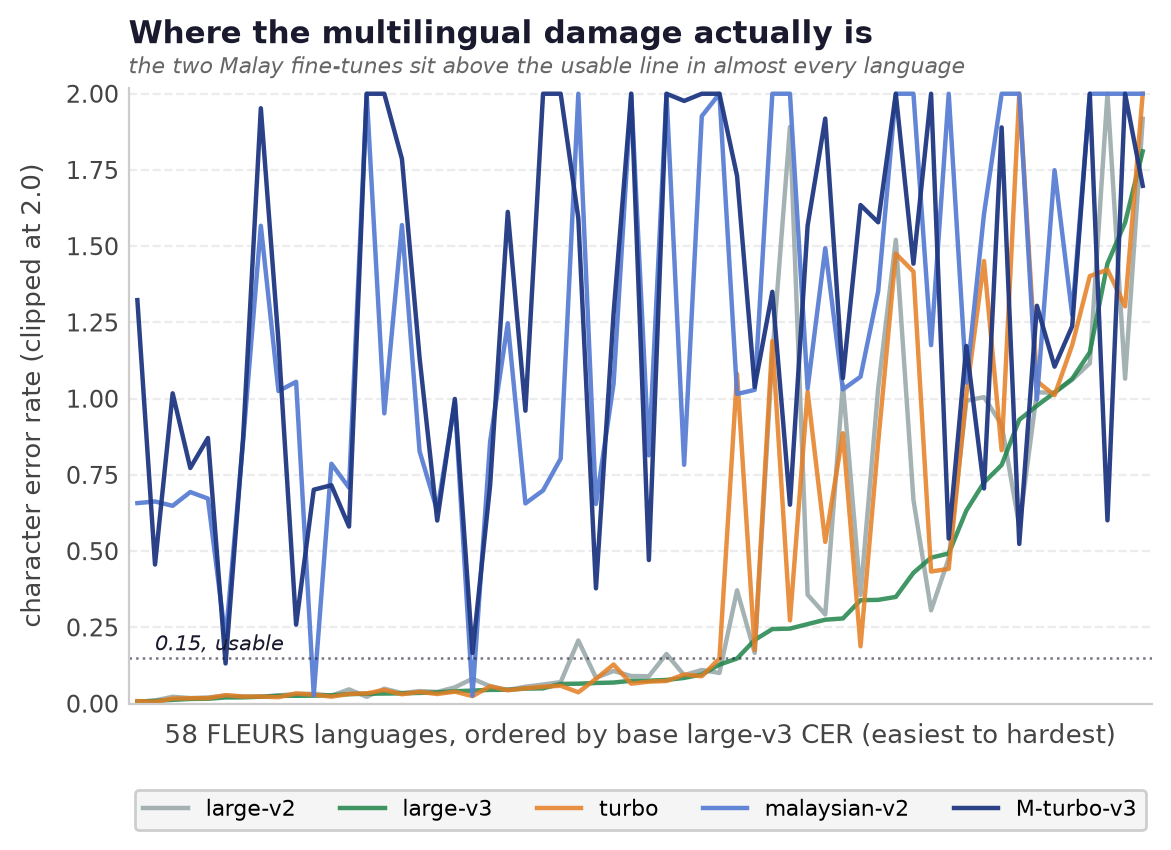
\includegraphics[width=0.86\linewidth]{img/fig_fleurs_per_lang.png}
  \caption{The same measurement language by language, ordered by base \texttt{large-v3}
  difficulty. Whisper genuinely cannot transcribe the right hand end: Amharic, Khmer and Somali
  sit above 1.4 for every checkpoint. The two Malay fine-tunes sit above the usable line almost
  everywhere, which is the damage LibriSpeech cannot report.}
  \label{fig:fleursperlang}
\end{figure}

\begin{figure}[tb]
  \centering
  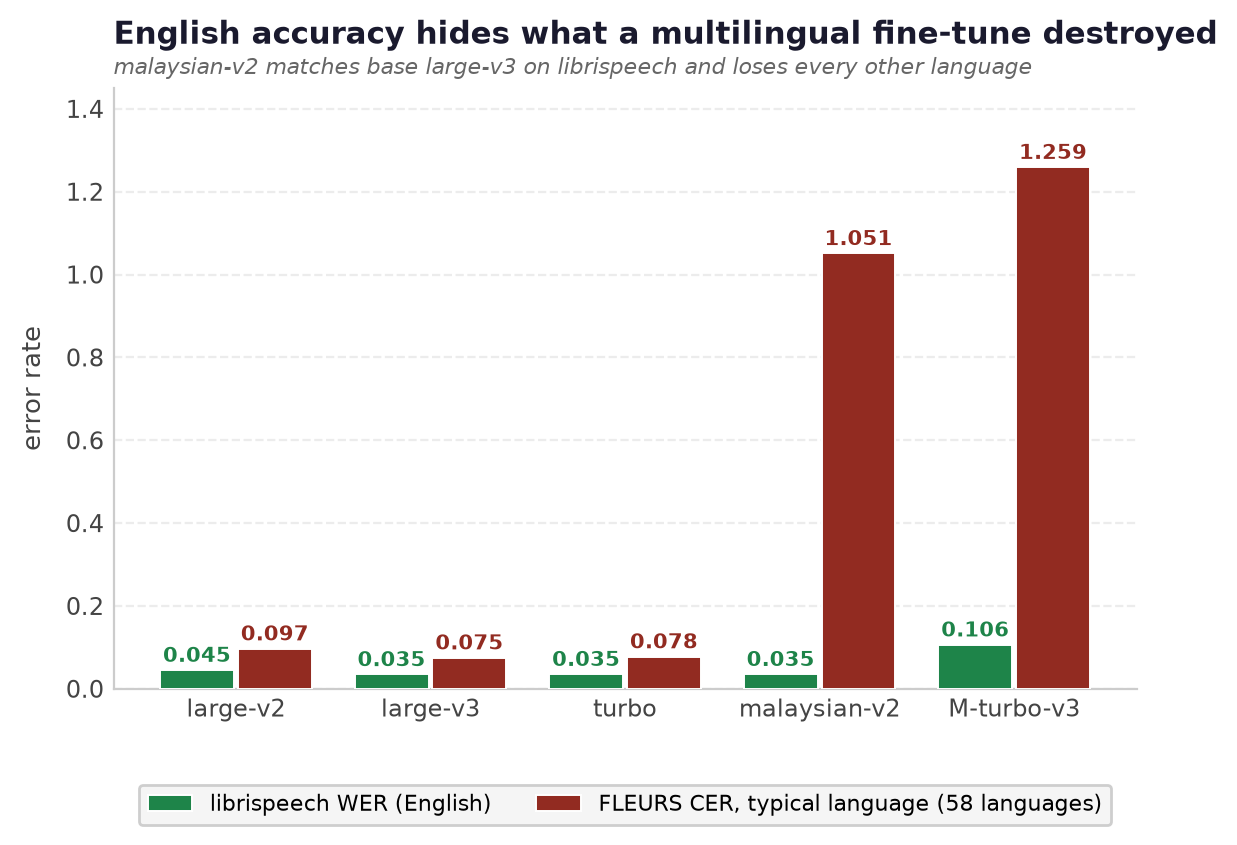
\includegraphics[width=0.86\linewidth]{img/fig_accuracy.png}
  \caption{English accuracy hides what a multilingual fine-tune destroyed. \texttt{malaysian-whisper-v2} matches base \texttt{large-v3} on LibriSpeech and returns character error rate 1.05 on the typical FLEURS language.}
  \label{fig:accuracy}
\end{figure}

\texttt{M-turbo-v3} looks broken in Table~\ref{tab:wer} and is not. Drop the roughly 1\% of
clips carrying a token run of six or more and \texttt{genuine} falls from 60.7\% to 33.9\%, and
\texttt{speech\_in\_noise} from 58.7\% to 25.6\%, the best in the table. One percent of clips
carries 27 points of word error rate. Looping is also what separates \texttt{turbo} from
\texttt{large-v3} on FLEURS, 4.7\% of clips against 0.9\%.

\subsection{The positive arm}

\begin{figure}[tb]
  \centering
  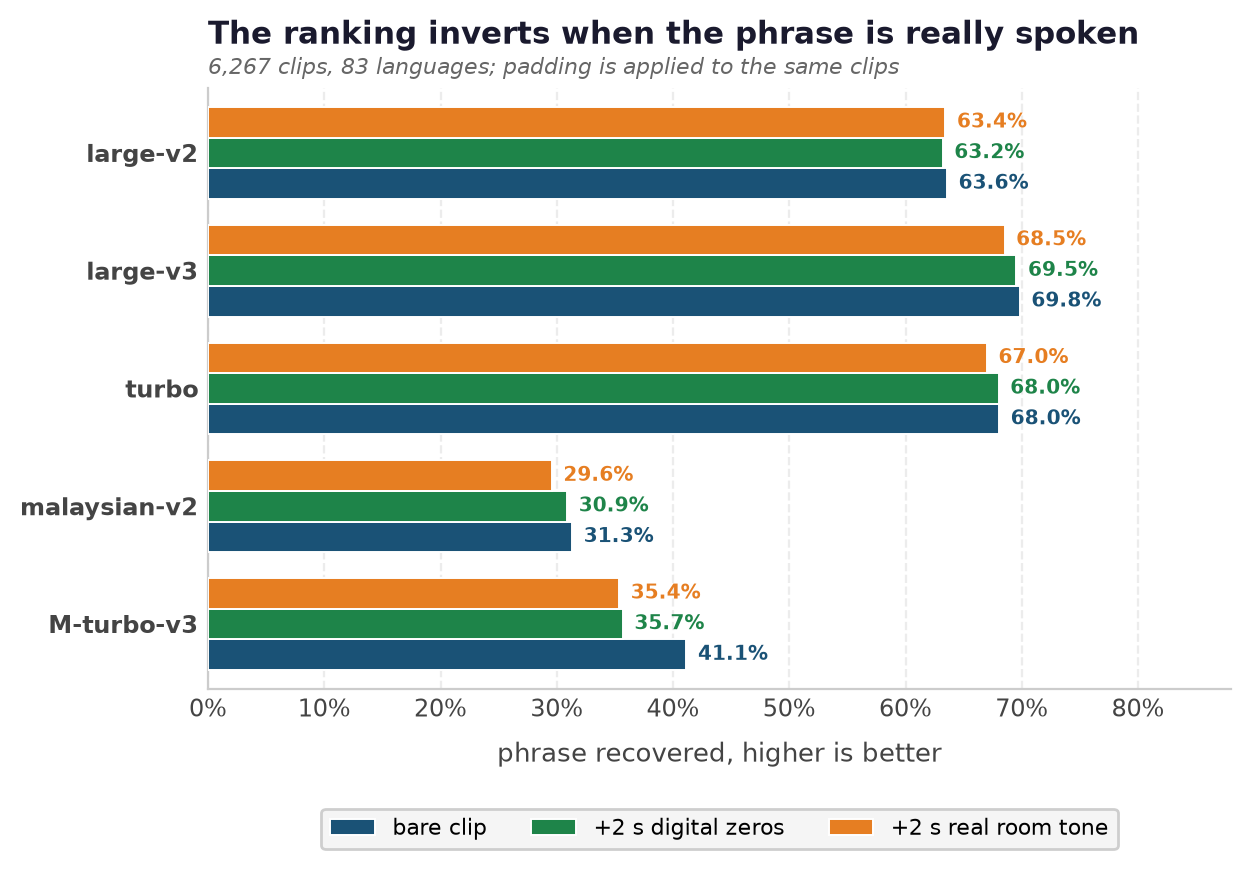
\includegraphics[width=0.86\linewidth]{img/fig_lexsynth_recovered.png}
  \caption{The ranking inverts when the phrase is really spoken. 6,267 clips in 83 languages, each run three ways. Padding is applied to the same clips, so each triple is a within-clip comparison.}
  \label{fig:lexsynth}
\end{figure}

\begin{table}[tb]
\centering
\caption{\texttt{lexicon\_synth} test split. Emitting the phrase is correct here.}
\label{tab:lexsynth}
\small
\begin{tabular}{lllrl}
\toprule
\textbf{model} & \textbf{recovered (bare to room tone)} & \textbf{median CER} & \textbf{mean CER} & \textbf{$>2\times$ output} \\
\midrule
\texttt{whisper-large-v2} & 63.6\% to 63.4\% & 0.125 & 0.378 to 0.384 & 0.6\% to 0.7\% \\
\textbf{\texttt{whisper-large-v3}} & \textbf{69.8\% to 68.5\%} & \textbf{0.089} & 0.288 to 0.302 & 0.2\% to 0.4\% \\
\texttt{whisper-large-v3-turbo} & 68.0\% to 67.0\% & 0.087 & 0.348 to 0.382 & 0.7\% to 0.9\% \\
\texttt{malaysian-whisper-v2} & 31.3\% to 29.6\% & 0.800 & 0.770 to \textbf{1.151} & 2.6\% to 3.7\% \\
\texttt{Malaysian-turbo-v3} & 41.1\% to 35.4\% & 0.385 & 1.508 to \textbf{3.749} & 3.0\% to 5.7\% \\
\bottomrule
\end{tabular}
\end{table}

\texttt{Malaysian-turbo-v3} wins every non-speech arm in Table~\ref{tab:nonspeech} and recovers
41.1\% of genuinely spoken phrases, against 69.8\% for \texttt{large-v3}. Its silence is a prior
against emitting text, not a detector. Report one side only and you will ship it.

Room tone costs the fine-tunes and not the base models. Same speech, two seconds of noise floor
on each side: \texttt{malaysian-v2} gains 0.38 mean character error rate,
\texttt{M-turbo-v3} gains 2.24, \texttt{large-v3} gains 0.014. Mean character error rate here is
a tail statistic. The median moves by hundredths while the mean triples, because 3\% to 6\% of
clips run past twice the phrase length.

\subsection{Results on wild audio}

\begin{figure}[tb]
  \centering
  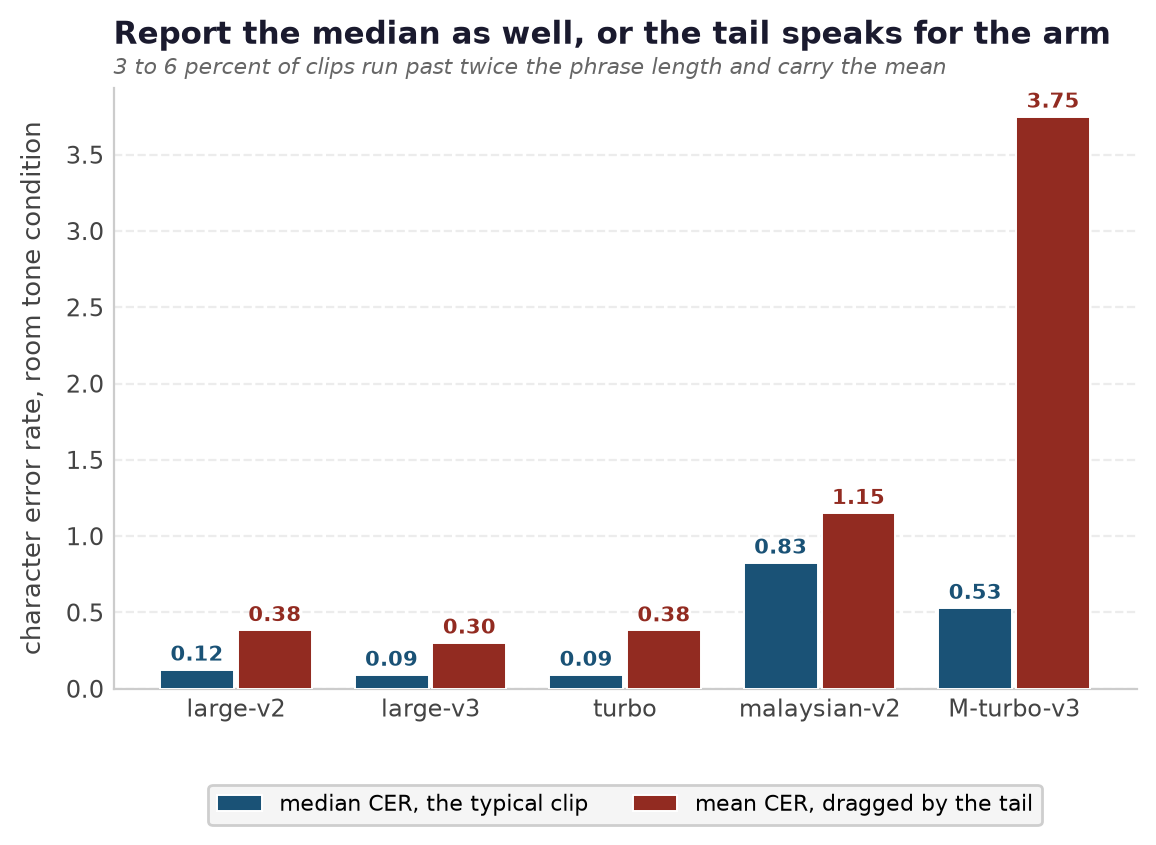
\includegraphics[width=0.86\linewidth]{img/fig_lexsynth_tail.png}
  \caption{Mean character error rate on the positive arm is a tail statistic. The median barely
  moves between checkpoints while the mean triples, because a few percent of clips run past
  twice the phrase length. Report both.}
  \label{fig:lexsynthtail}
\end{figure}

\begin{figure}[tb]
  \centering
  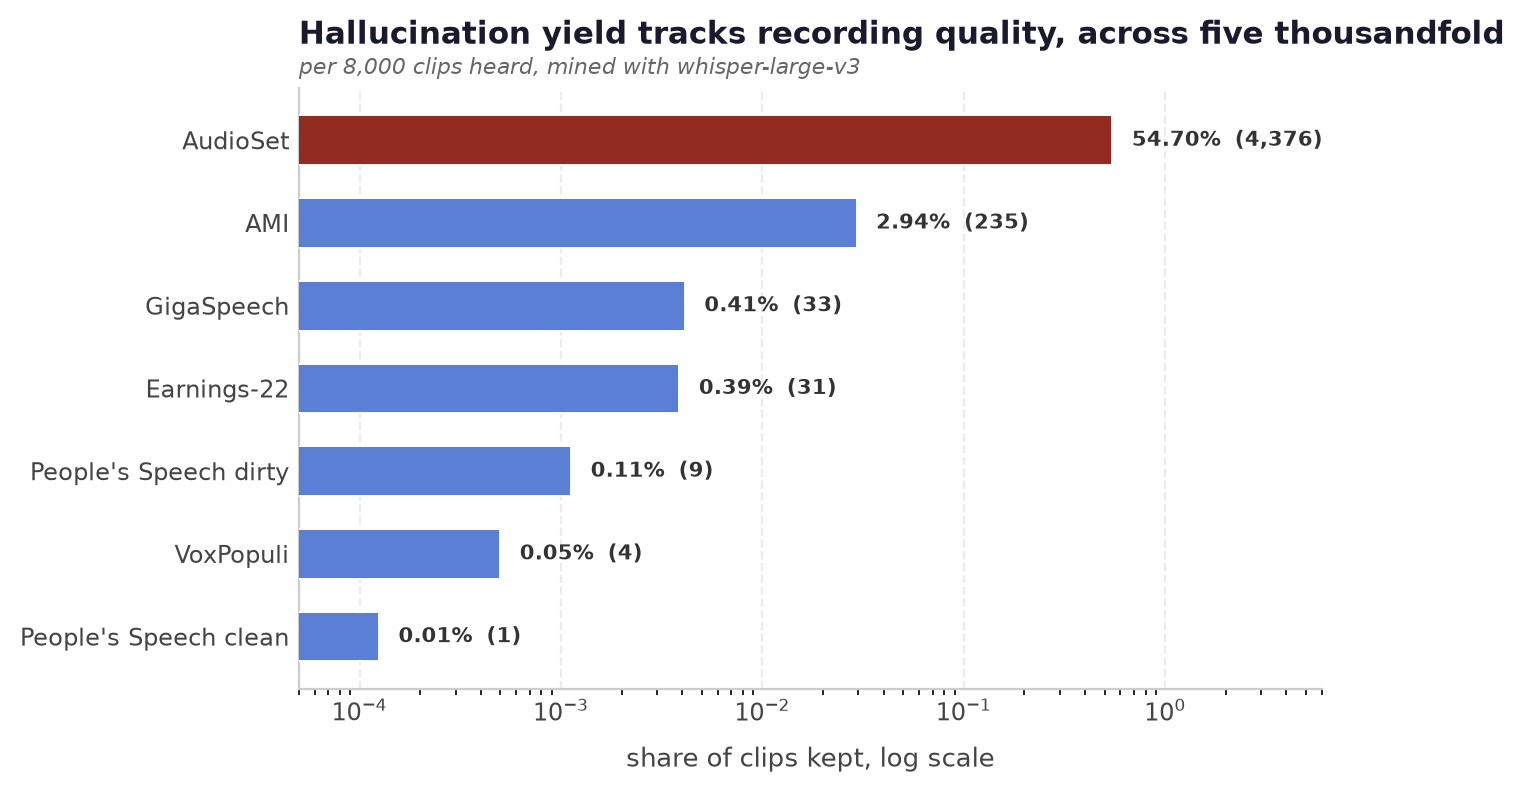
\includegraphics[width=0.86\linewidth]{img/fig_wild_yield.png}
  \caption{Hallucination yield by corpus, per 8,000 clips heard, on a log scale. Curated corpora barely fail. GigaSpeech is the right material and still yields 0.41\%, because its segments are cut to speech.}
  \label{fig:wildyield}
\end{figure}

On 4,421 clips that a voice activity detector confirms contain no speech, every OpenAI
checkpoint emits words on 100\% of them. \texttt{Malaysian-turbo-v3} emits words on 8.5\%. Of
those outputs, 53.6\% for \texttt{large-v3} and 72.1\% for \texttt{turbo} are exactly a phrase
from the lexicon, against roughly 18\% to 22\% on speech clips from the same corpus. The
blocklist works, but only once the audio is already known to be blank.

Most wild loops are model-specific. On clips mined because \texttt{large-v3} looped,
\texttt{turbo} loops on 17.2\%. A loop corpus mined with one model is not a fair loop benchmark
for another.

\begin{figure}[tb]
  \centering
  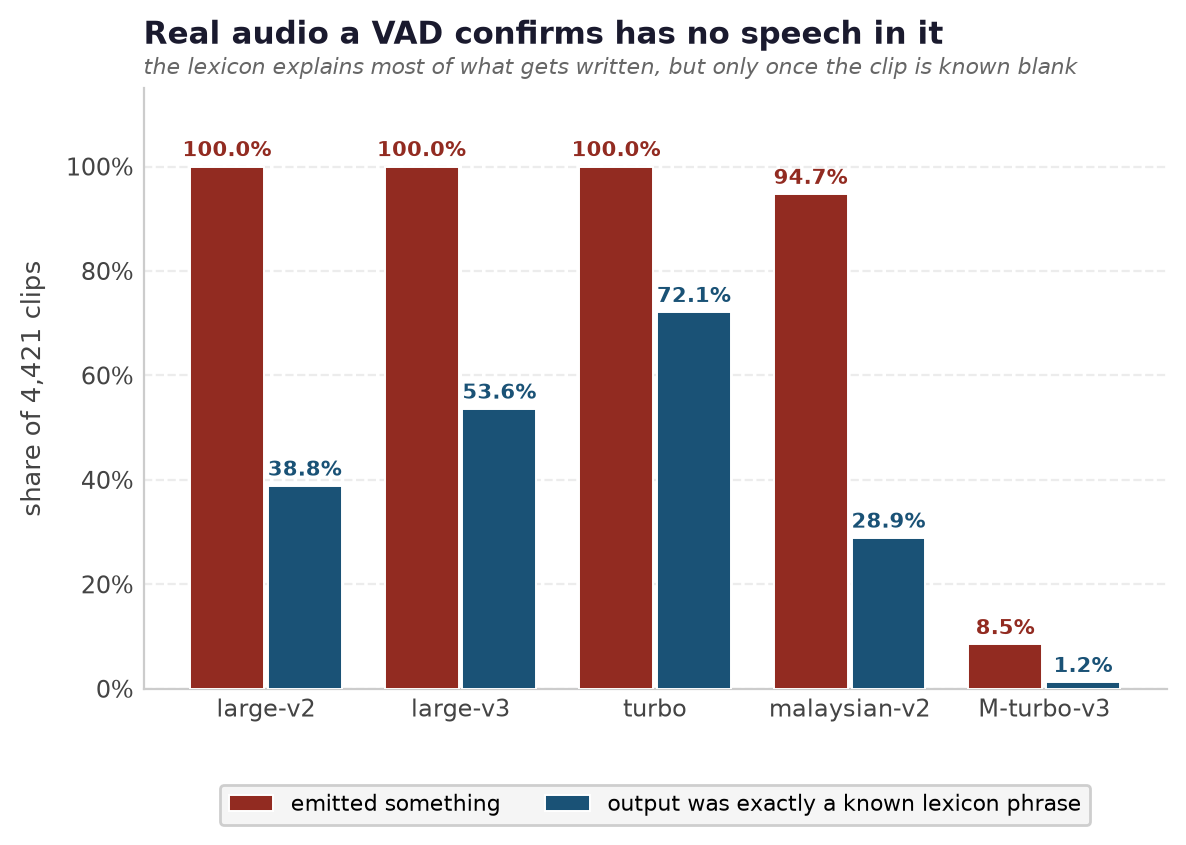
\includegraphics[width=0.86\linewidth]{img/fig_wild_blank.png}
  \caption{Real audio that a voice activity detector confirms has no speech in it. Every OpenAI
  checkpoint writes something on all 4,421 clips. Most of what they write is a phrase from the
  lexicon, which is what makes a blocklist work, but only once the clip is already known to be
  blank.}
  \label{fig:wildblank}
\end{figure}

\section{Lexicon}
\label{sec:lexicon}

Hallucinations repeat themselves. \texttt{thank you for watching}, \texttt{so}, the Russian
\texttt{Prodolzhenie sleduet...} (``to be continued''), and the Malay
\texttt{terima kasih kerana menonton} appear over and over on audio containing none of them. We merged four public sources with our own mining
into 40,891 phrases across 100 languages.

The lexicon is the bridge between the two halves of this work. Read one way it is a blocklist.
Read the other way it is a list of sentences the model must still be able to transcribe when
somebody genuinely says them, which is exactly the training signal that is missing.

It needs filtering before use. It contains Whisper's own loop artefacts captured as phrases.
One entry is a single Gujarati character repeated seven times. These wreck character error rate
comparisons, one of them produced a CER of 22.9. We drop any entry that is a single repeated
token or has two or fewer distinct characters.

It also needs a frequency cut. Of 39,476 queued entries, 35,594 were observed exactly once, and
27,974 of those run five words or longer. They are raw recognition fragments, not phrases:
\texttt{0073a this vehicle s got 72 00 miles on it 3 5l v engine}. Synthesising those is
pointless, because the round trip fails by construction on digits and truncation. Two
independent text-to-speech systems score character error rate near 1.0 on them, which is the
signal that the input is at fault rather than the generator. We synthesise entries observed at
least twice: 3,882 entries across 85 languages, median two words.

\section{Synthesis}

To turn the lexicon into training data we need each phrase spoken aloud, in its own language, in
more than one voice. That is a text-to-speech problem, and the choice of system matters more
than it looks.

\subsection{Choosing a generator}

\begin{figure}[tb]
  \centering
  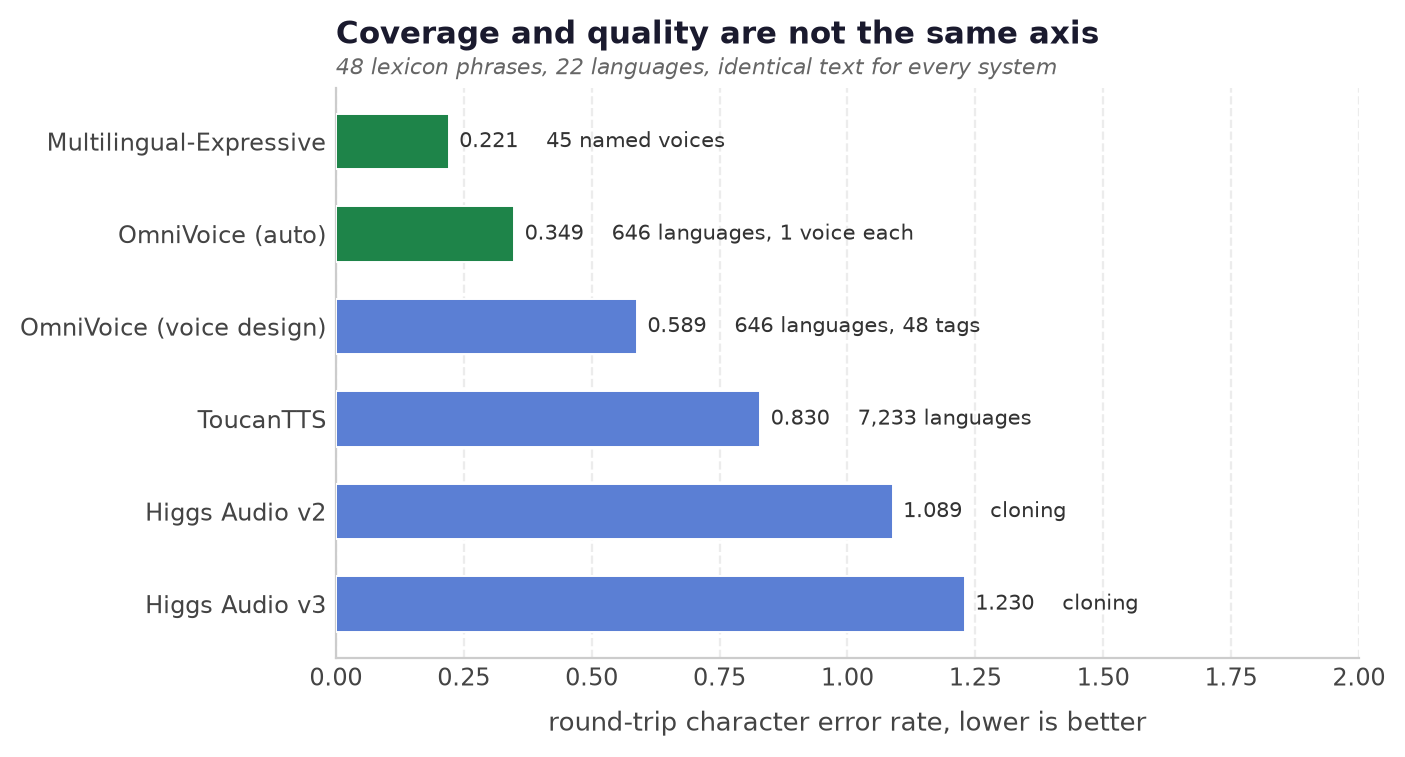
\includegraphics[width=0.86\linewidth]{img/fig_tts.png}
  \caption{Text-to-speech candidates on 48 lexicon phrases in 22 languages, identical text, scored by recognition round trip. Coverage and quality are not the same axis.}
  \label{fig:tts}
\end{figure}

\begin{table}[tb]
\centering
\caption{Text-to-speech candidates. Round-trip character error rate, lower is better.}
\label{tab:tts}
\small
\begin{tabular}{lrrrllll}
\toprule
 & \textbf{mean CER} & \textbf{median} & \textbf{wins} & \textbf{languages} & \textbf{voices} \\
\midrule
Multilingual-Expressive-TTS-1.7B & \textbf{0.221} & \textbf{0.000} & \textbf{16} & untagged & 45 named \\
OmniVoice (auto) & 0.349 & 0.018 & 2 & \textbf{646} & \textbf{1 per language} \\
OmniVoice (voice design) & 0.589 & 0.062 & 3 & \textbf{646} & 48 tags \\
ToucanTTS & 0.830 & 0.586 & 0 & \textbf{7{,}233} & sampled from a GAN \\
Higgs Audio v2 & 1.089 & 0.713 & 0 & untagged & cloning \\
Higgs Audio v3 & 1.230 & 0.483 & 1 & 82/100 & cloning \\
\bottomrule
\end{tabular}
\end{table}

Coverage and quality are not the same axis. ToucanTTS covers 7,233 languages and wins nothing.
OmniVoice covers 646 and is the only system whose coverage is enumerable, so it drives the
hundred-language sweep, with Multilingual-Expressive handling Malay, English, Chinese and Tamil.

\subsection{Voice diversity}

\begin{figure}[tb]
  \centering
  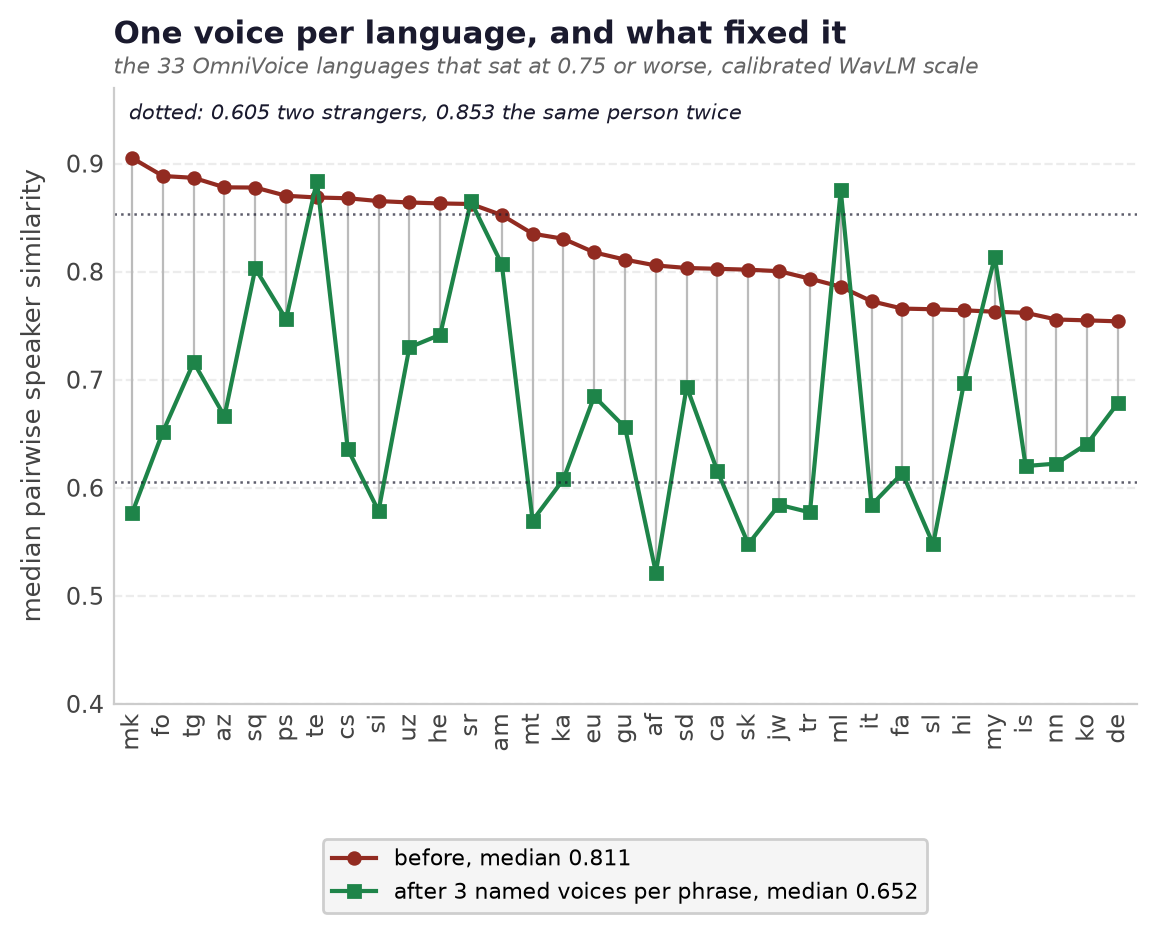
\includegraphics[width=0.86\linewidth]{img/fig_voice_diversity.png}
  \caption{One voice per language, and what fixed it. Pairwise speaker similarity on a calibrated scale where 0.605 is two strangers and 0.853 is two clips of the same person.}
  \label{fig:diversity}
\end{figure}

OmniVoice takes no speaker argument, so every clip it produces carries an empty voice field. We
measured what that means with WavLM speaker embeddings \citep{chen2021wavlm} on a calibrated
scale: 33 of its 74 languages sat at a median pairwise cosine of 0.75 or worse. One voice per
language. A corpus built that way teaches the model one speaker's phrase, not the phrase.

The obvious fix, reference cloning, is the wrong one.

\begin{table}[tb]
\centering
\caption{Two routes to distinct voices, probed on the same 4 languages, 24 phrases and 4 voices.
Lower cosine means better separated voices.}
\label{tab:diversity}
\small
\begin{tabular}{llll}
\toprule
\textbf{route} & \textbf{yield mk / gu / it} & \textbf{median CER} & \textbf{different-voice cosine} \\
\midrule
\textbf{Multilingual-Expressive, speaker name} & \textbf{86\% / 80\% / 79\%} & 0.07 / 0.17 / 0.00 & \textbf{0.65 / 0.64 / 0.58} \\
OmniVoice, reference cloning & 46\% / 68\% / 53\% & 0.32 / 0.25 / 0.26 & 0.68 / 0.72 / 0.69 \\
auto mode, for reference & 89\% / 73\% / 83\% & 0.02 / 0.11 / 0.00 & 0.91 / 0.81 / 0.77 \\
\bottomrule
\end{tabular}
\end{table}

Cloning costs about half the yield and separates the voices less well than simply naming a
speaker. So we topped up 26 languages rather than replacing them: three named voices per phrase,
auto-mode clips kept. 12,190 of 15,675 new clips passed the quality gate, 77.8\%, and the median
collapsed language moved from 0.81 to 0.63.

\subsection{Voice conversion}

\begin{figure}[tb]
  \centering
  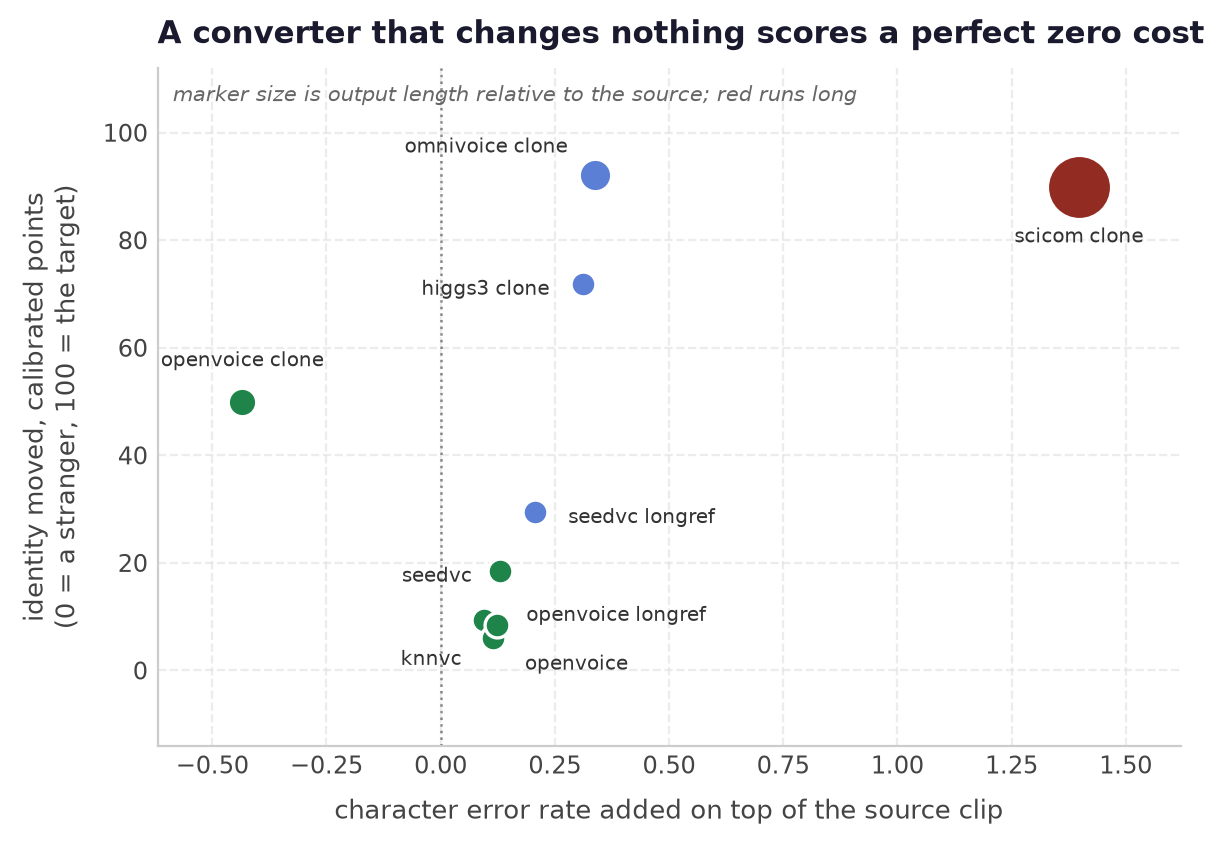
\includegraphics[width=0.86\linewidth]{img/fig_vc.png}
  \caption{Voice conversion candidates. Character error rate added on top of the source clip against how far the voice actually moved. A converter that returns its input scores a perfect zero cost and is worthless, which is why the vertical axis is here at all.}
  \label{fig:vc}
\end{figure}

Character error rate alone picks the wrong winner here, because a converter that returns its
input unchanged scores a perfect zero degradation and is worthless. We report the cost added on
top of the source clip, similarity to the target and to the source on the same calibrated
scale, and the gap between them, which is the conversion that actually happened.

\subsection{Quality gate}

Every synthesised clip passes a recognition round trip: the recogniser must recover the phrase,
and the clip must run about as long as the phrase should take. The gate is per language and
anchored to the judge's own floor, which is Whisper's character error rate on real FLEURS speech
in that language. A language where the judge itself scores 0.88, as it does on Burmese, cannot
be held to a 0.25 gate. Nine such languages are excluded rather than scored.

The final corpus is 29,112 clips in 83 languages, 22,845 train and 6,267 test, 15.8 hours, 92\%
non-English.

\section{Training sweep}
\label{sec:sweep}

\subsection{Setup}

We fine-tune \texttt{whisper-large-v3} with LoRA \citep{hu2021lora} and with full fine-tuning.
The target for a blank clip is the empty transcript under that clip's language token, which is
what teaches ``no words here'' rather than ``emit something short''. The four prompt tokens are
masked out of the loss, so loss falls only on the transcript and the final end-of-text token.

\begin{table}[tb]
\centering
\caption{Training sets. Everything is disjoint from the benchmark by construction and every
test split stays held out.}
\label{tab:trainsets}
\small
\begin{tabular}{lrrll}
\toprule
\textbf{source} & \textbf{clips} & \textbf{hours} & \textbf{target} & \textbf{teaches} \\
\midrule
\texttt{corpus} nonspeech (FSD50K \texttt{dev}) & 16{,}983 & 33.3 & empty & noise means say nothing \\
\texttt{corpus} music (FMA shards 2-12) & 7{,}170 & 58.3 & empty & music means say nothing \\
\texttt{corpus} Malay speech (Emilia \citep{he2024emilia}) & 5{,}801 & 14.8 & transcript & keep accuracy \\
\texttt{corpus} reduplication & 2{,}514 & 4.0 & exact repeats & do not run away \\
\texttt{corpus} silence & 59 & 0.7 & empty & room tone means say nothing \\
\texttt{lexicon\_synth} train & 22{,}845 & 12.5 & the phrase & the phrase is real, transcribe it \\
\texttt{wild} train & 3{,}656 & 9.6 & empty & real noisy audio means say nothing \\
\bottomrule
\end{tabular}
\end{table}

\subsection{Mixes}

The sweep answers a paired question, and both halves are run at every configuration.

\begin{enumerate}
\item Without the synthetic lexicon, does fine-tuning improve hallucination and repetition on
real audio?
\item With the synthetic lexicon, does it improve them further, and what does it cost?
\end{enumerate}

Two mixes, identical except for the synthetic positives.

\begin{table}[tb]
\centering
\caption{The paired mixes. \texttt{no\_synth} is \texttt{all} with \texttt{lexicon\_synth}
removed and nothing else changed.}
\label{tab:mixes}
\small
\begin{tabular}{lrrl}
\toprule
\textbf{mix} & \textbf{clips} & \textbf{blank share} & \textbf{contains \texttt{lexicon\_synth}} \\
\midrule
\texttt{no\_synth} & 36{,}183 & 77\% & no \\
\texttt{all} & 59{,}028 & 47\% & yes, 22{,}845 clips \\
\bottomrule
\end{tabular}
\end{table}

Removing the synthetic positives also moves the blank share from 47\% to 77\%. That is not a
confound to be stripped out, it is the mechanism. The synthetic positives are the counterweight,
and removing them necessarily makes the mix more blank-dominated.

\subsection{Grid}

Twelve configurations per mix, twenty-four runs in total. LoRA alpha tracks twice the rank so
rank is the only thing that varies. Adapters cover the attention projections and the two
feed-forward layers, because those hold most of the parameters in a Whisper block. Full
fine-tunes use batch 4 with 4 accumulation steps to hold the same 16 clips per optimiser step as
LoRA's 8 with 2, so effective batch size does not confound the comparison.

\begin{table}[tb]
\centering
\caption{The grid. 1e-3 is absent on purpose, see below.}
\label{tab:grid}
\small
\begin{tabular}{llrl}
\toprule
\textbf{method} & \textbf{rank / alpha} & \textbf{trainable params} & \textbf{learning rates} \\
\midrule
LoRA & 32 / 64 & 57.7 M (3.6\%) & 1e-4, 2e-4, 5e-4 \\
LoRA & 64 / 128 & 115.3 M (7.0\%) & 1e-4, 2e-4, 5e-4 \\
LoRA & 128 / 256 & 230.7 M (13.0\%) & 1e-4, 2e-4, 5e-4 \\
full fine-tune & & 1{,}574.9 M (100\%) & 5e-6, 1e-5, 2e-5 \\
\bottomrule
\end{tabular}
\end{table}

Every run is trained for 1,000 steps with 50 warmup steps in bf16, then scored on the complete
benchmark: the eight published arms, the synthetic positives, the wild test split, and FLEURS.

\textbf{Control the optimiser before attributing anything to the data.} Our first sweep ran at
1e-3. The \texttt{corpus} mix finished at loss 9.76 while mixes containing the same clips
finished at 1.1 to 1.2, which reads as evidence that a blank-heavy mix is bad. It is not. The
same mix at 2e-4 converges cleanly to 0.64. The checkpoint from the diverged run hallucinates on
100\% of silence and 100\% of music, which is a broken optimiser, not a data result.

\subsection{Results}

% RESULTS PLACEHOLDER: filled from bench/readme_tables.py once the 24 runs finish.

\section{Limitations}

The positive pool is largely synthetic. It is 52\% synthetic text-to-speech and 23\% read prose,
and only 25\% is real conversational speech, which is Sarawak dialect. A model tuned on
synthesised phrases may be learning something about the generator as well as about the phrases.

There is no telephony condition. Everything is 16 kHz, and a great deal of production audio is
8 kHz narrowband.

Chinese and Tamil positives are close to absent, 11 and 4 clips.

The \texttt{silence} arm is 42 clips, so its resolution is 2.4 percentage points per clip.
Differences of a few points on that arm are noise. The \texttt{music} arm may contain singing,
since its source labels vocals as unknown. \texttt{nonspeech} is the label-verified alternative
and should be preferred when the two disagree.

\texttt{speech\_in\_noise} is synthetic mixing, so the signal-to-noise ratio is exact but there
is no Lombard effect and no channel.

The synthetic corpus was filtered using \texttt{whisper-large-v3} with the language forced, so
that checkpoint is scored partly on clips it already agreed with. This flatters it against
\texttt{large-v2} and \texttt{turbo}. It does not explain a thirty point gap to the Malay
fine-tunes.

\section{Future work}

The decoder-side ablation is designed and not run: 34 configurations of beam width, temperature
fallback, repetition and presence penalties, and the interaction between those and a fine-tuned
checkpoint. The interesting question is whether a model trained to stop still needs the knobs.

Stage two of the sweep is the winning configuration applied to
\texttt{whisper-large-v3-turbo}, which is the checkpoint most people actually serve and the one
with the worst repetition profile of the three base models.

Two languages, Sinhala and Malagasy, have no FLEURS configuration, so they have no judge floor
and fall back to a flat gate that accepts almost nothing. They need a floor measured from
another corpus before their phrases can be synthesised reliably.

Finally, the wild pool should grow. AudioSet yields more than half of what it is asked for, so
the bottleneck is not availability, it is compute and storage. A wild benchmark an order of
magnitude larger would let hallucination be measured per acoustic condition rather than in
aggregate.

\section{Acknowledgement}

This work was carried out at Scicom (MSC) Berhad. The author thanks Scicom for the compute and
for the time to publish the negative results alongside the positive ones.

\bibliographystyle{plainnat}
\bibliography{neurips_2023}

\end{document}
